\documentclass{beamer}
%
% Choose how your presentation looks.
% For more themes, color themes and font themes, see:
% http://deic.uab.es/~iblanes/beamer_gallery/index_by_theme.html
%
\mode<presentation>
{
  \usetheme{Madrid}      % or try Darmstadt, Madrid, Warsaw, ...
  \usecolortheme{seahorse} % or try albatross, beaver, crane, ...
  \usefonttheme{serif}  % or try serif, structurebold, ...
  \setbeamertemplate{navigation symbols}{}
  \setbeamertemplate{caption}[numbered]
  \usepackage{amsmath}
  \usepackage{tcolorbox}
  \usepackage[export]{adjustbox}
  \tcbuselibrary{most}
  \usepackage{amsmath}  % conflicts with \oiint
  \usepackage{arydshln}
  \usepackage{tikz}
  \usetikzlibrary{plotmarks}
  \usepackage{pgfplots}
  \newcommand{\Ivec}[1]{\mbox{\boldmath $#1$}}
    \usepackage[normalem]{ulem}
    % \usepackage{tipa}
    \newcommand{\git}{\texttt{\textbf{git}}\xspace}
    \usepackage{listings}
} 


\definecolor{myblue}{RGB}{65,105,225} 
\definecolor{myorange}{RGB}{250,190,0}

\setbeamercolor{structure}{fg=white,bg=myorange}
\setbeamercolor*{palette primary}{fg=myblue,bg=myorange}
\setbeamercolor*{palette secondary}{fg=white,bg=myblue}
\setbeamercolor*{palette tertiary}{bg=myblue,fg=white}
\setbeamercolor*{palette quaternary}{fg=white,bg=myorange!50}

\setbeamercolor{frametitle}{fg=black!90!myblue}

\setbeamercolor{section in head/foot}{fg=white,bg=myblue}
\setbeamercolor{author in head/foot}{fg=black,bg=myorange}
\setbeamercolor{title in head/foot}{fg=white,bg=myblue}

\setbeamertemplate{navigation symbols}{}

\setbeamertemplate{itemize/enumerate body begin}{\large}
\setbeamertemplate{itemize/enumerate subbody begin}{\large}


\defbeamertemplate*{headline}{mytheme}
{%
  \begin{beamercolorbox}[ht=2.25ex,dp=3.75ex]{section in head/foot}
    \insertnavigation{\paperwidth}
  \end{beamercolorbox}%
}%

\defbeamertemplate*{footline}{mytheme}
{
  \leavevmode%
  \hbox{%
  \begin{beamercolorbox}[wd=.5\paperwidth,ht=2.25ex,dp=1ex,right]{author in head/foot}%
    \usebeamerfont{author in head/foot}\insertshortauthor\hspace*{2em}
  \end{beamercolorbox}%
  \begin{beamercolorbox}[wd=.5\paperwidth,ht=2.25ex,dp=1ex,left]{title in head/foot}%
    \usebeamerfont{title in head/foot}\hspace*{2em}\insertshortsubtitle\hspace*{2em}
    \insertframenumber{} / \inserttotalframenumber
  \end{beamercolorbox}}%
  \vskip0pt%
}

\usepackage[english]{babel}
\usepackage[utf8x]{inputenc}
\usepackage{xcolor}
\usepackage{listings}
\usepackage{pgf}  
\usepackage{textpos}
\usepackage{tabulary}
\usepackage{scrextend}
\usepackage{hyperref}
\usepackage{setspace}
\usepackage{rotating}
\lstset
{
    language=[LaTeX]TeX,
    breaklines=true,
    basicstyle=\tt\scriptsize,
    %commentstyle=\color{green}
    keywordstyle=\color{blue},
    %stringstyle=\color{black}
    identifierstyle=\color{magenta},
}
\newcommand{\bftt}[1]{\textbf{\texttt{#1}}}
%\newcommand{\comment}[1]{{\color[HTML]{008080}\textit{\textbf{\texttt{#1}}}}}
\newcommand{\cmd}[1]{{\color[HTML]{008000}\bftt{#1}}}
\newcommand{\bs}{\char`\\}
\newcommand{\cmdbs}[1]{\cmd{\bs#1}}
\newcommand{\lcb}{\char '173}
\newcommand{\rcb}{\char '175}
\newcommand{\cmdbegin}[1]{\cmdbs{begin\lcb}\bftt{#1}\cmd{\rcb}}
\newcommand{\cmdend}[1]{\cmdbs{end\lcb}\bftt{#1}\cmd{\rcb}}

\newcommand{\wllogo}{\textbf{Overleaf}}

\usepackage{hyperref}
\hypersetup{
    colorlinks=true,
    linkcolor=blue,
    filecolor=magenta,      
    urlcolor=cyan,
    pdftitle={Overleaf Example},
    pdfpagemode=FullScreen,
    }

\urlstyle{same}

% this is where the example source files are loaded from
% do not include a trailing slash
\newcommand{\fileuri}{https://raw.githubusercontent.com/GiancarloSucci/UniBo.IDSEPC.A2022/main/A2022.IDSEPCLaTeX/}

\newcommand{\perche}{perch\'{e}}
\newcommand{\affinche}{affinch\'{e}}
\newcommand{\se}{s\'{e}}
\newcommand{\a}{\`{a}}
\newcommand{\est}{\`{e}}

\usepackage{stackengine}
\def\Ruble{\stackengine{.67ex}{%
  \stackengine{.48ex}{\textsf{P}}{\rule{.8ex}{.12ex}\kern.6ex}{O}{r}{F}{F}{L}%
  }{\rule{.8ex}{.12ex}\kern.6ex}{O}{r}{F}{F}{L}\kern-.1ex}



%----------------------------------------------------------------------------------------
%	TITLE PAGE
%----------------------------------------------------------------------------------------
\title[L02]{Introduzione alla data science e al pensiero computazionale\\
Lezione 9: Regressione lineare} % The short title appears at the bottom of every slide, the full title is only on the title page

\author[{\tiny Giancarlo Succi }]{Giancarlo Succi\\\\ Dipartimento di Informatica -- Scienza e Ingegneria\\Universit\`{a} di Bologna\\
\bftt{g.succi@unibo.it}
} % Your name
\institute[unibo] % Your institution as it will appear on the bottom of every slide, may be shorthand to save space

\date{} % Date, can be changed to a custom date

\setbeamertemplate{navigation symbols}{}
\AtBeginSection[]
{
        \begin{frame}<beamer>{Outline}
                \tableofcontents[currentsection]
        \end{frame}
}

\begin{document}
\begin{frame}
\titlepage % Print the title page as the first slide

\end{frame}

%=============================================

\addtobeamertemplate{frametitle}{}{%
\begin{textblock*}{10mm}(-0.01mm,-0.95cm)

\includegraphics[width=0.9cm]{unibo-logo.png}
\end{textblock*}}

%=============================================

\begin{frame}
{\centerline{Linear Regression -- Problem 1}}
%Define here the mathematical definition of the OLS linear regression, as the line that minimized the square error
Suppose that:
\begin{itemize}
\item  I want to relate two random scalar phenomena, $X$ and $Y$, to identify the relationships existing between them,
\item I can measure their values several times $i$, so I can have a set of pairs ($x_i$,$y_i$) with $i$ spanning the interval of observation, say $i \in [0 \ldots{} n-1]$
\end{itemize}

\begin{table}[h!]
\small
  \begin{center}
    \begin{tabular}{|c|c|c|}      
    \hline
     \textit{i} & \textbf{X} & \textbf{Y} \\
    \hline    \hline
	\textit{0} &1 & 3 \\
	\textit{1} &2 & 4 \\
	\textit{2} &5 & 4 \\
	\textit{3} &6 & -1 \\
	\textit{4} &7 & 5 \\
	\textit{5} &9 & 8 \\
	\textit{6} &12 & 9 \\
	\textit{7} &13 & 9 \\ \hline
    \end{tabular}
  \end{center}
\end{table}


\end{frame}

\begin{frame}
{\centerline{Linear Regression -- Problem 2}}
%Define here the mathematical definition of the OLS linear regression, as the line that minimized the square error
Using a simple and common approach, I may try to build a relationship between the two phenomena.
However:
\begin{itemize}
\item  What kind of relationships I am going to look for?
\item How do I build it?
\end{itemize}

\end{frame}

\begin{frame}
{\centerline{Linear Regression -- Problem 3}}
%Define here the mathematical definition of the OLS linear regression, as the line that minimized the square error

In other words, I have this set of points:

\begin{center}
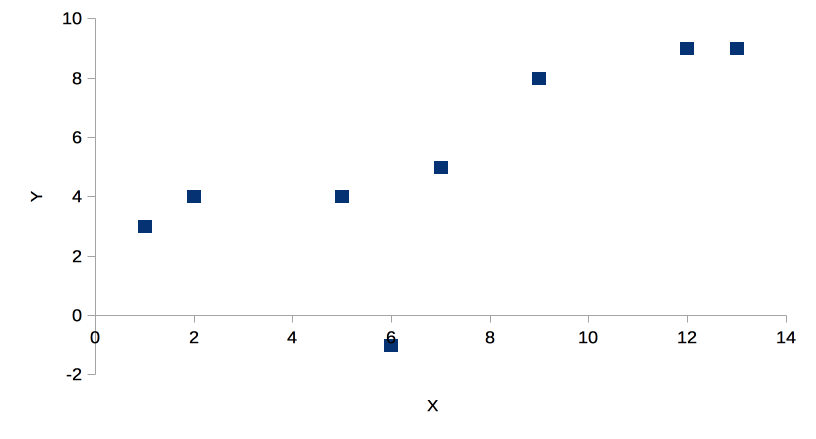
\includegraphics[width=10cm]{A2022.IDSEPC.RegressioneLineare/LinearRegression_Points.png}
\end{center}

\end{frame}

\begin{frame}
{\centerline{Linear Regression -- Problem 4}}
%Define here the mathematical definition of the OLS linear regression, as the line that minimized the square error

How can I build a line that represent the relationships between these two sets?

\begin{center}
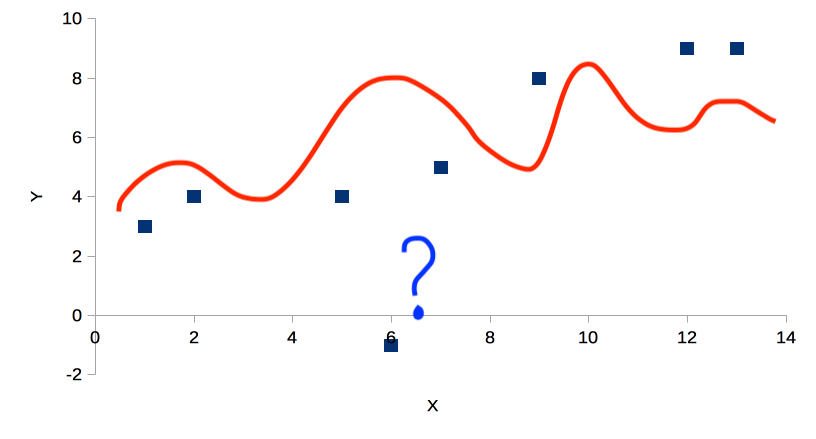
\includegraphics[width=10cm]{A2022.IDSEPC.RegressioneLineare/LinearRegression_Lines.png}
\end{center}



\end{frame}

%----------------------------------------------------------------------------------------
\begin{frame}
{\centerline{Linear Regression -- Definition}}
%Define here the mathematical definition of the OLS linear regression, as the line that minimized the square error
We need to define:
\begin{itemize}
\item A \textcolor{red}{mean function} that represents the relationship that I hypothesize between the phenomena $X$ and $Y$\\
\item A \textcolor{red}{cost-minimization function} to define the parameters of the mean function
\end{itemize}
\vspace*{0.5cm}
We will use initially:
\begin{itemize}
\item As \textcolor{red}{mean function} the simple line\\
\item As \textcolor{red}{cost function} the square of the errors between the modeled values and the real values
\end{itemize}
\vspace*{0.5cm}
We define \textcolor{red}{Ordinary Least Squares (OLS) Linear Regression} as a simple line that minimizes a square error between modelled values and real values.
\end{frame}

\begin{frame}
{\centerline{Linear Regression -- Goal}}
%Define here the mathematical definition of the OLS linear regression, as the line that minimized the square error

This is what we would like to build:

\begin{center}
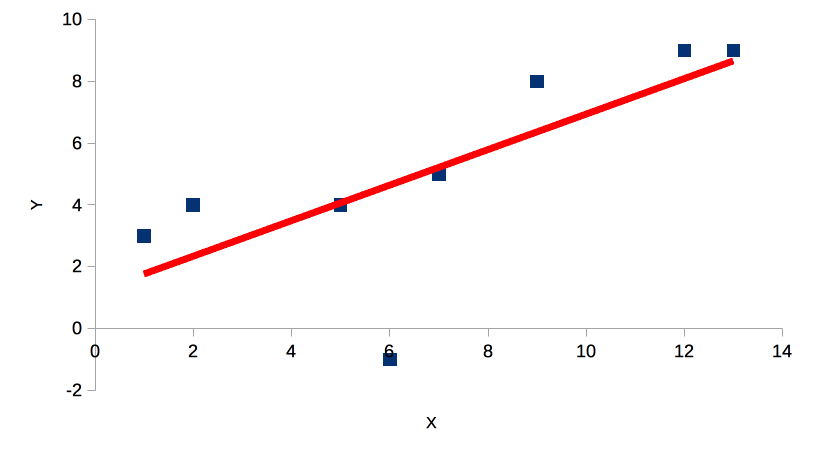
\includegraphics[width=12cm]{A2022.IDSEPC.RegressioneLineare/LinearRegression_OLS.png}
\end{center}



\end{frame}

\begin{frame}
{\centerline{Linear Regression -- Alternative Goal 1}}
%Define here the mathematical definition of the OLS linear regression, as the line that minimized the square error

But we could have used as a mean function a cubic function:

\begin{center}
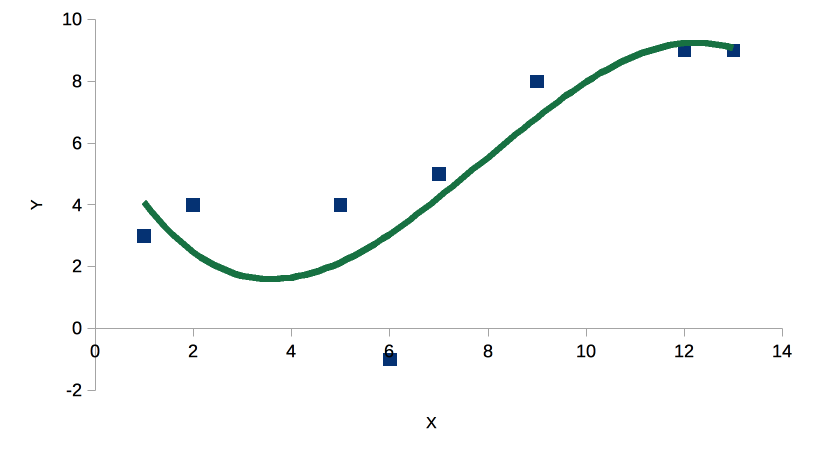
\includegraphics[width=12cm]{A2022.IDSEPC.RegressioneLineare/LinearRegression_Degree3.png}
\end{center}

\end{frame}

\begin{frame}
{\centerline{Linear Regression -- Alternative Goal 2}}
%Define here the mathematical definition of the OLS linear regression, as the line that minimized the square error

But we could have used as a mean function a fifth order function:

\begin{center}
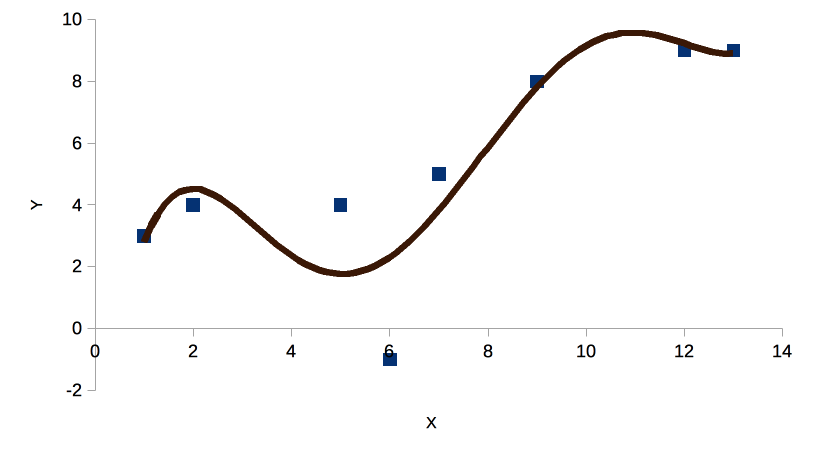
\includegraphics[width=12cm]{A2022.IDSEPC.RegressioneLineare/LinearRegression_Degree5.png}
\end{center}

\end{frame}

\begin{frame}
{\centerline{Linear Regression -- All Goals}}
%Define here the mathematical definition of the OLS linear regression, as the line that minimized the square error

What are the differences between all these 3?

\begin{center}
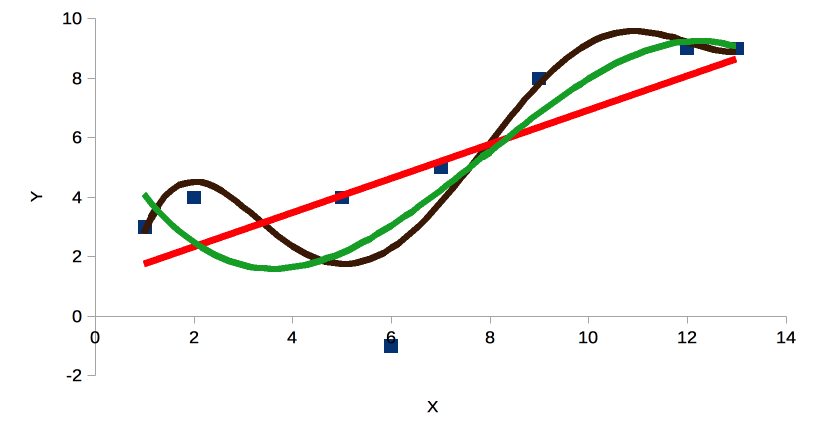
\includegraphics[width=12cm]{A2022.IDSEPC.RegressioneLineare/LinearRegression_O35.png}
\end{center}

\end{frame}




\begin{frame}
{\centerline{Linear Regression -- Formula 1}}
I want to build a model of the kind:

$$ Y = \theta_0 + \theta_1 X $$

Where $X$ and $Y$ are the phenomena that we are measuring.\\
\vspace*{0.3cm}

Note:
\begin{itemize}
\item we know that there is no line passing for $n$ arbitrary points with $n \leq 3$
\item we need to introduce an approximation
$$ \hat{Y} = \theta_0 + \theta_1 \hat{X} + \epsilon $$
\item in our case $\epsilon$ is the error that is introduced by the approximation
\item as we said, our cost function, our distance from the model, will be the square of the error $\epsilon^2$
\item $ \theta_0$ and $\theta_1$ are called the \textcolor{red}{regression coefficients}
\end{itemize}

\end{frame}

\begin{frame}
{\centerline{Linear Regression -- Formula 2}}
Altogether:
\begin{itemize}
\item we have a set of pairs ($x_i$,$y_i$)  with $i \in [0 \ldots{} n-1]$
\item we want to build $n$ linear equations of the kind (the mean function):
$$ y_i = \theta_0 + \theta_1 x_i + \epsilon_i $$
\item and we start with an approximation of the kind:
$$ \hat{y}_i = \theta_0 + \theta_1 x_i  $$
\end{itemize}

\end{frame}

\begin{frame}
{\centerline{Linear Regression -- Formula 3}}
Altogether:
\begin{itemize}
\item our goal is to compute  $\theta_0$ and $\theta_1$ that minimize the quadratic error (the cost function)
$$ \sum_{i=0}^{n-1}\epsilon_i^2  $$

\item notice that:
\begin{itemize}
\item we will denote as ($x_i$,$y_i$) the original data
\item we will denote as ($\hat{x}_i$,$\hat{y}_i$) the approximation that we obtain in the linear regression
\item $x_i$ and $\hat{x}_i$ are the same
\item \textcolor{red}{there could be errors in the slides and you get extra credits by finding them}
\end{itemize}
\end{itemize}

\end{frame}


\begin{frame}
{\centerline{Linear Regression -- Computation 1}}
\begin{itemize}
\item Since 
$$ y_i = \theta_0 + \theta_1 x_i + \epsilon_i $$
\item therefore
$$\epsilon_i  = y_i - \theta_0 - \theta_1 x_i $$
\item we need to minimize:
$$ \sum_{i=0}^{n-1}\epsilon_i^2  = \sum_{i=0}^{n-1}(y_i - \theta_0 - \theta_1 x_i)^2  $$
\item we need to zero the two partial derivatives:
$$ \frac{\partial \sum_{i=0}^{n-1}(y_i - \theta_0 - \theta_1 x_i)^2}{\partial \theta_i}$$
\item so we have to solve two simple equations and then to check the Hessian
\end{itemize}

\end{frame}


\begin{frame}
{\centerline{Linear Regression -- Computation for $\theta_0$}}

$$ \frac{\partial \sum_{i=0}^{n-1}(y_i - \theta_0 - \theta_1 x_i)^2}{\partial \theta_0} =  0 \Rightarrow$$ \\
$$ 2 \sum_{i=0}^{n-1}(y_i - \theta_0 - \theta_1 x_i) = 0 \Rightarrow$$ \\
$$ \sum_{i=0}^{n-1}(y_i - \theta_0 - \theta_1 x_i) = 0 $$

\end{frame}

\begin{frame}
{\centerline{Linear Regression -- Computation for $\theta_1$}}

$$ \frac{\partial \sum_{i=0}^{n-1}(y_i - \theta_0 - \theta_1 x_i)^2}{\partial \theta_1} =  0 \Rightarrow$$ \\
$$ 2 \sum_{i=0}^{n-1}x_i(y_i - \theta_0 - \theta_1 x_i) = 0 \Rightarrow$$ \\
$$ \sum_{i=0}^{n-1}x_i(y_i - \theta_0 - \theta_1 x_i) = 0 $$

\end{frame}

\begin{frame}
{\centerline{Linear Regression -- From the first equation}}

From the first equation:

$$ \sum_{i=0}^{n-1}(\theta_0) = \sum_{i=0}^{n-1}( y_i - \theta_1 x_i)  \Rightarrow $$ \\
$$ \sum_{i=0}^{n-1}(\theta_0) = \sum_{i=0}^{n-1}( y_i ) - \theta_1 \sum_{i=0}^{n-1}(x_i)  \Rightarrow $$\\
$$ n \theta_0 = n \bar{y} - n \theta_1 \bar{x}  \Rightarrow $$\\
$$ \theta_0 = \bar{y} - \theta_1 \bar{x}  $$



\end{frame}

\begin{frame}
{\centerline{Linear Regression -- In the second equation}}
$$ \sum_{i=0}^{n-1}x_i(y_i - \theta_0 - \theta_1 x_i) = 0   \Rightarrow $$

$$ \sum_{i=0}^{n-1}x_iy_i - \theta_0 \sum_{i=0}^{n-1}x_i - \theta_1 \sum_{i=0}^{n-1}x_i^2 = 0 \Rightarrow $$

$$ \sum_{i=0}^{n-1}x_iy_i - n \theta_0 \bar{x}  - n \theta_1 \bar{x^2} = 0 \Rightarrow $$


\end{frame}

\begin{frame}
{\centerline{Linear Regression -- Combining the result}}

Substituting $ \theta_0  = \bar{y} - \theta_1 \bar{x} $:

$$ \sum_{i=0}^{n-1}x_iy_i - n (\bar{y} - \theta_1 \bar{x}) \bar{x}  - n \theta_1 \bar{x^2} = 0 \Rightarrow $$

$$ \sum_{i=0}^{n-1}x_i y_i - n \bar{y}\bar{x} + n \theta_1 \bar{x}^2  - n \theta_1 \bar{x^2} = 0$$

$$ n \theta_1 (\bar{x^2}  - \bar{x}^2 ) = \sum_{i=0}^{n-1}x_i y_i - n \bar{y}\bar{x} $$
\end{frame}

\begin{frame}
{\centerline{Linear Regression -- Final step}}

$$ \theta_1  = \frac {\sum_{i=0}^{n-1}x_i y_i - n \bar{y}\bar{x}} {n (\bar{x^2}  - \bar{x}^2 ) } $$
\vspace*{0.2cm}

$$ \theta_1  = \frac { \frac {\sum_{i=0}^{n-1}x_i y_i}{n}  - \bar{y}\bar{x}} { (\bar{x^2}  - \bar{x}^2 ) } $$
\vspace*{0.2cm}

$$ \theta_1  = \frac { Cov(x,y)} { Var(x) } $$

Which we can also write as:

$$\theta_1 = \frac{\sum_{i=0}^{n-1}(x_i-\bar{x})(y_i-\bar{y})}{\sum_{i=0}^{n-1}(x_i-\bar{x})^2}$$


\end{frame}

\begin{frame}
{\centerline{Going back to our exercise... }}

Using the formula above we obtain that for the following dataset:

\begin{table}[h!]
\small
  \begin{center}
    \begin{tabular}{|c|c|c|}      
    \hline
     \textit{i} & \textbf{X} & \textbf{Y} \\
    \hline    \hline
	\textit{0} &1 & 3 \\
	\textit{1} &2 & 4 \\
	\textit{2} &5 & 4 \\
	\textit{3} &6 & -1 \\
	\textit{4} &7 & 5 \\
	\textit{5} &9 & 8 \\
	\textit{6} &12 & 9 \\
	\textit{7} &13 & 9 \\ \hline
    \end{tabular}
  \end{center}
\end{table}


We have an equation:
$$ \hat{Y} = \theta_0 + \theta_1 \hat{X} $$
with:
\begin{itemize}
\item $\theta_0$ = 1.179
\item $\theta_1$ = 0.574

\end{itemize}

\end{frame}

\begin{frame}
{\centerline{Our model }}


\begin{table}[h!]
\small
  \begin{center}
    \begin{tabular}{|c|c|c|c|c|}      
    \hline
     \textit{i} & \textbf{X} & \textbf{Y} & \textbf{$\hat{Y}$} & \textbf{$\epsilon$}\\
    \hline    \hline
	\textit{0} &1 & 3 & 1.753 & 1.247 \\
	\textit{1} &2 & 4 & 2.327 & 1.673 \\
	\textit{2} &5 & 4  & 4.049 & -0.049\\
	\textit{3} &6 & -1 & 4.623 & -5.623 \\
	\textit{4} &7 & 5  & 5.197 & -0.197\\
	\textit{5} &9 & 8  & 6.345 & 1.655\\
	\textit{6} &12 & 9  & 8.067 & 0.933\\
	\textit{7} &13 & 9  & 8.641 & 0.359\\ \hline
    \end{tabular}
  \end{center}
\end{table}


\end{frame}

\begin{frame}
{\centerline{Linear Regression -- Exercise}}

Build a linear regression for the following dataset:
\begin{center}
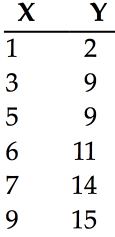
\includegraphics[width=2cm]{A2022.IDSEPC.RegressioneLineare/points-1.png}
\end{center}

\end{frame}
%=====%=====%=====%=====%=====%=====%=====%=====%=====
\begin{frame}
{\centerline{Linear Regression -- Exercise}}

\begin{center}
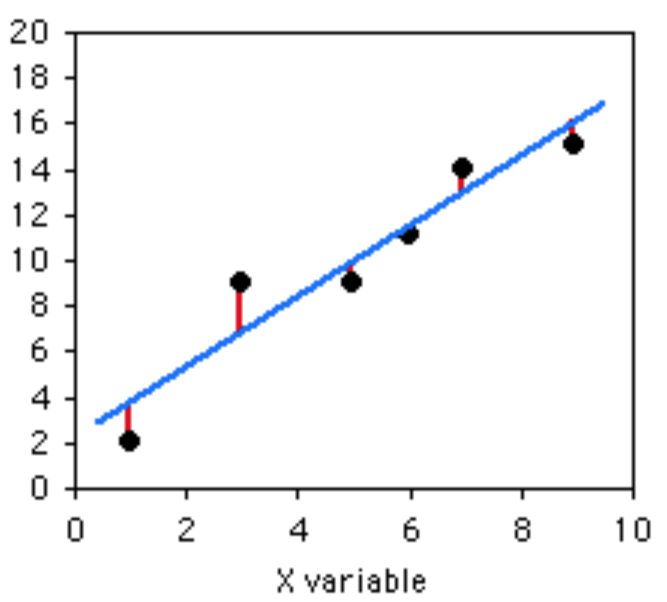
\includegraphics[width=6cm]{A2022.IDSEPC.RegressioneLineare/points-2.png}   
\end{center}


\end{frame}




\begin{frame}
{\centerline{Linear Regression -- Exercise}}

The regression equation for these numbers is $\hat{y}=2.0286+1.5429x$. Now, fill the blanks using such equation and calculate the sum of squared deviations (last column).
\small
\begin{table}[]
\centering
\begin{tabular}{l | l | l | l| l} 
\hline
x & y & Predicted y ($\hat{y}$) & Deviate from predicted (abs.) & Squared deviate \\
\hline

1 & 2 &  &  &  \\
3 & 9 &  &  &  \\
5 & 9 &  &  &  \\
6 & 11 &  &  &  \\
7 & 14 & &  &  \\
9 & 15 &  &  &  \\

\hline

\end{tabular}
\end{table}
\end{frame}

%=====%=====%=====%=====%=====%=====%=====%=====%=====

\begin{frame}
{\centerline{Linear Regression -- Exercise}}

Results. The sum of squared deviations: 10.8
\small
\begin{table}[]
\centering
\begin{tabular}{l | l | l | l| l} 
\hline
x & y & Predicted y ($\hat{y}$) & Deviate from predicted (abs.) & Squared deviate \\
\hline

1 & 2 & 3.57 & 1.57 & 2.46 \\
3 & 9 & 6.66 & 2.34 & 5.48 \\
5 & 9 & 9.74 & 0.74 & 0.55 \\
6 & 11 & 11.29 & 0.29 & 0.08 \\
7 & 14 & 12.83 & 1.17 & 1.37 \\
9 & 15 & 15.91 & 0.91 & 0.83 \\

\hline

\end{tabular}
\end{table}
\end{frame}


\begin{frame}
{\centerline{Linear Regression -- Modeling}}
In fact, we might think to use linear regression to model phenomena, assuming a linear dependence between input (the collected parameters) and output. 

Here are some “real world” examples (w.r.t. certain assumptions):

\begin{itemize}
\item - Impact of SAT Score (or GPA) on College Admissions;
\item - Impact of product price on number of sales;
\item - Impact of rainfall amount on the number of fruits yielded;
\item - Impact of blood alcohol content on coordination.
\end{itemize}

\end{frame}


\begin{frame}
{\centerline{Linear Regression -- Evaluation}}
We can evaluate the quality of linear regression, i.e. assess how good the model for the data that we have:

\begin{itemize}
\item - by the sum of squares of residuals;
\item - by the coefficient of determination.
\end{itemize}



\end{frame}


\begin{frame}
{\centerline{The sum of squared errors}}

The sum of squares of residuals, also called the residual sum of squares:

$$SS_{res} = \sum_i (y_i - \hat{y}_i)^2$$

In the case above $SS_{res}$ is equal to 39.751672.

\end{frame}

\begin{frame}
{\centerline{The coefficient of determination ($R^2$)}}

The coefficient of determination describes the proportion of variance of the dependent variable explained by the regression model. If the regression model is “perfect”, $SS_{res}$ is zero, and $R^2$ is 1.

$$R^2 = 1 - \frac{SS_{res}}{SS_{tot}}$$

The total sum of squares:

$$SS_{tot} = \sum_i (y_i - \bar{y})^2$$

where 
$$\bar{y}=\frac{1}{n}\sum_{i=1}^n y_i$$

\end{frame}

\begin{frame}
{\centerline{In the example above}}

$$SS_{tot} = \sum_i (y_i - \bar{y})^2 = 82.875 $$

Remember that:

$$SS_{res} = \sum_i (y_i - \hat{y}_i)^2 = 39.751672$$

Therefore:

$$R^2 = 1 - \frac{SS_{res}}{SS_{tot}} = 1 - \frac{39.751672}{82.875} =  0.5203$$

\end{frame}

\begin{frame}
{\centerline{Coefficient of determination ($R^2$)}}


\begin{center}
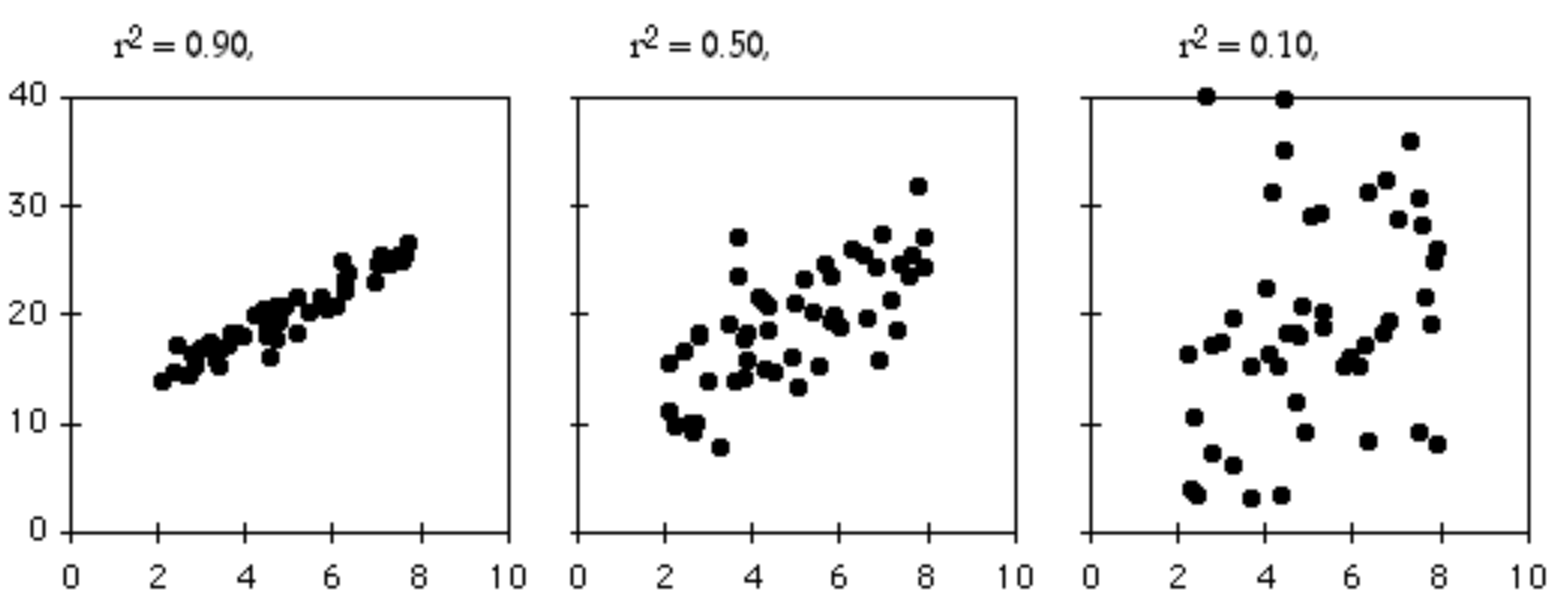
\includegraphics[width=12cm]{A2022.IDSEPC.RegressioneLineare/r2.png}   
\end{center}
\end{frame}

\begin{frame}
{\centerline{Multivariate Linear Regression }}

\begin{itemize}
\item The ``X'' variable is often called ``feature'' in machine learning.
\item Indeed, we could have multiple features, say, $n$.
\item If we also have $m$ observations, we could build a system of $m$ equations of the kind:
$$ y_i = \boldsymbol \theta^T \cdot \boldsymbol x_i + \epsilon_i, i=1\ldots m$$
\item and then we will build our linear regression (approximation) as:
$$ \hat{y_i} = \boldsymbol \theta^T \cdot \boldsymbol{\hat{x_i}}, i=1\ldots m$$

\item where $\boldsymbol x_i$ and  $\boldsymbol{\hat{x_i}}$-- are vectors of $n+1$ features for the i-th observation
\end{itemize}

\textbf{Question:} Why here we use $n+1$?
\end{frame}

\begin{frame}
{\centerline{A closed-form solution of Linear Regression }}

To find the value of $\boldsymbol \theta$, there is a closed-form solution, a mathematical equation that gives the result directly.  

This is called the \textbf{Normal Equation}:

$$\theta = (\boldsymbol X \cdot \boldsymbol X^T)^{-1} \cdot \boldsymbol X^T \cdot \boldsymbol y$$


\end{frame}

\begin{frame}
{\centerline{Derivation of the closed-form solution  (1/4) }}

\begin{itemize}
\item We start considering a set of $m$ equations of the form:
$$ \hat{y_i} = \boldsymbol \theta^T \boldsymbol x_i, i=1\ldots m$$
\subitem  where $\boldsymbol x_i$ has dimension $n+1$
\item We move all the model in matrix format:
$$  \hat{\boldsymbol y} = \boldsymbol X \cdot \boldsymbol \theta   $$
\subitem Notice that $\hat{\boldsymbol y}$ and $\boldsymbol y$ have dimension (m,1), $\boldsymbol X$ (m,n+1), and $\theta$  (n+1,1). $\boldsymbol X \cdot \boldsymbol \theta$ has therefore dimension (m,1) as it should be.

\item The error vector $ {\boldsymbol \epsilon}$ is defined for each pair as:

$$ {\boldsymbol \epsilon} = \hat{\boldsymbol y} - \boldsymbol y = \boldsymbol X \cdot \boldsymbol \theta - {\boldsymbol y} $$

\item And the square of the error is:
$$  (\boldsymbol X \cdot \boldsymbol \theta - \boldsymbol y)^T (\boldsymbol X \cdot \boldsymbol \theta - \boldsymbol y) $$

\end{itemize}

\end{frame}

\begin{frame}
{\centerline{Derivation of the closed-form solution  (2/4) }}

\begin{itemize}
\item To determine the values of the parameters we take the partial derivatives and we null them:
$$ \frac{ \partial  (\boldsymbol X \cdot \boldsymbol \theta - \boldsymbol y)^T (\boldsymbol X \cdot \boldsymbol \theta - \boldsymbol y)} { \partial \boldsymbol \theta} = 0 $$
\item Now we evaluate:
$$ \frac{ \partial  (\boldsymbol X \cdot \boldsymbol \theta - \boldsymbol y)^T (\boldsymbol X \cdot \boldsymbol \theta - \boldsymbol y)} { \partial \boldsymbol \theta} = $$
 $$ = \frac{\partial (
 (\boldsymbol X \cdot \boldsymbol \theta)^T (\boldsymbol X \cdot \boldsymbol \theta) -
 (\boldsymbol X \cdot \boldsymbol \theta)^T \boldsymbol y -
 \boldsymbol y^T\boldsymbol X \cdot \boldsymbol \theta +
  \boldsymbol y^T \boldsymbol y
 )}
 { \partial \boldsymbol \theta} = $$
  $$ = \frac{\partial (
 (\boldsymbol X \cdot \boldsymbol \theta)^T (\boldsymbol X \cdot \boldsymbol \theta) -
 2 (\boldsymbol X \cdot \boldsymbol \theta)^T \boldsymbol y +
  \boldsymbol y^T \boldsymbol y
 )}
 { \partial \boldsymbol \theta} $$

\end{itemize}

\end{frame}

\begin{frame}
{\centerline{Derivation of the closed-form solution  (3/4) }}

\begin{itemize}
\item Now we can consider that:
  $$ \frac{\partial (  \boldsymbol y^T \boldsymbol y )}
 { \partial \boldsymbol \theta} = 0 $$
 \item that:
  $$ \frac{\partial (
  (\boldsymbol X \cdot \boldsymbol \theta)^T \boldsymbol y
 )}
 { \partial \boldsymbol \theta} = \boldsymbol X^T \boldsymbol y$$
 \item Notice that $\boldsymbol X^T \boldsymbol y$ has dimension (n+1,m) $\cdot$ (m,1), that is, (n+1,1).

 \item and finally that:
  $$ \frac{\partial (
 (\boldsymbol X \cdot \boldsymbol \theta)^T (\boldsymbol X \cdot \boldsymbol \theta) )}
 { \partial \boldsymbol \theta} = 2  \boldsymbol X^T  \boldsymbol X \boldsymbol \theta $$
 \item Notice that $\boldsymbol X^T \boldsymbol X \boldsymbol \theta$ has dimension (n+1,m) $\cdot$ (m,n+1)  $\cdot$ (n+1,1), that is, (n+1,1) as it should be.

\end{itemize}

\end{frame}

\begin{frame}
{\centerline{Derivation of the closed-form solution (4/4) }}

\begin{itemize}
\item Substituting the results in the original formula:
  $$ 2  \boldsymbol X^T  \boldsymbol X \boldsymbol \theta - 2 \boldsymbol X^T \boldsymbol y = 0 \Rightarrow $$
  
    $$ \boldsymbol X^T  \boldsymbol X \boldsymbol \theta = \boldsymbol X^T \boldsymbol y  \Rightarrow $$
    
  \item Notice that $\boldsymbol X^T \boldsymbol X $ has dimension (n+1,m) $\cdot$ (m,n+1), that is, (n+1,n+1). Notice that m $\gg$ n, so we \textit{hope} that $\boldsymbol X^T \boldsymbol X $ is invertible.

    
        $$ \boldsymbol \theta = (\boldsymbol X^T  \boldsymbol X)^{-1}  \boldsymbol X^T \boldsymbol y  $$
        
\item QED.

\end{itemize}

\end{frame}

%--------------%%--------------%%--------------%%--------------%%--------------%%--------------%


% \begin{frame}
% {\centerline{\small  Linear Regression -- Computational complexity}}
% Discuss the computational complexity of linear regression
% \end{frame}


% \begin{frame}
% {\centerline{Linear Regression -- Approximation}}
% Discuss gradient descent
% \end{frame}

%--------------%%--------------%%--------------%%--------------%%--------------%%--------------%

\begin{frame}
{\centerline{Computational complexity}}

The Normal Equation computes the inverse of $X^T \cdot X$, which is an n x n matrix (where n is the number of features). 
\newline

The computational complexity of inverting such a matrix is typically about $O( n^{2.4})$ to $O( n^3)$ (depending on the implementation). 
\newline

In other words, if you double the number of features, you multiply the computation time by roughly $2^{2.4} = 5.3$ to $2^3 = 8$.

\end{frame}
%--------------%%--------------%%--------------%%--------------%%--------------%%--------------%

%--------------%%--------------%%--------------%%--------------%%--------------%%--------------%

\begin{frame}
{\centerline{Linear Regression -- Approximation}}

\textbf{Gradient Descent} is a very generic optimization algorithm capable of finding optimal solutions to a wide range of problems. The general idea of Gradient Descent is to tweak parameters iteratively in order to minimize a cost function.

\begin{center}
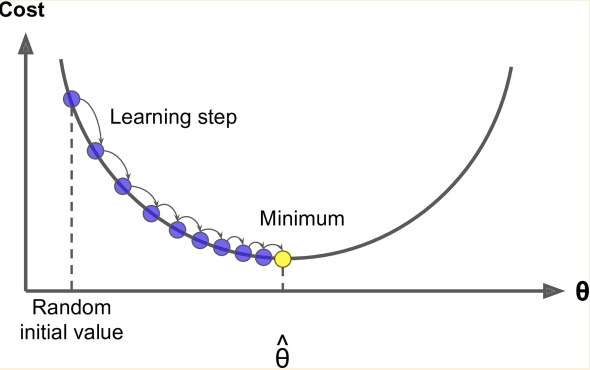
\includegraphics[width=8cm]{A2022.IDSEPC.RegressioneLineare/gd-1.png}
\end{center}


\end{frame}
%--------------%%--------------%%--------------%%--------------%%--------------%%--------------%

%--------------%%--------------%%--------------%%--------------%%--------------%%--------------%

\begin{frame}
{\centerline{Gradient Descent -  Computation }}


To implement Gradient Descent, you need to compute the gradient of the MSE cost function with regards to each model parameter $\theta_j$.

Mean squared error (MSE) cost function for a Linear Regression model:

$$MSE (\theta) = \frac{1}{m}\sum_{k=1}^{m} (\boldsymbol \theta^T \cdot \boldsymbol x^{(k)} - \boldsymbol y^{(k)})^2$$

$x^{(k)}$ - k-th observation vector ($x^{(k)}$ is an n-dimensional vector)



\end{frame}
%--------------%%--------------%%--------------%%--------------%%--------------%%--------------%


\begin{frame}
{\centerline{Gradient Descent -  Computation }}


To implement Gradient Descent, you need to compute the gradient of the MSE cost function with regards to each model parameter $\theta_j$.

$$\frac{\partial}{\partial \theta_j}MSE(\theta) = \frac{2}{m} \sum_{i=1}^{m}(\theta^T \cdot \boldsymbol x^{(i)} - \boldsymbol y^{(i)}  ) x_j^{(i)}$$
\end{frame}
%--------------%%--------------%%--------------%%--------------%%--------------%%--------------%

%--------------%%--------------%%--------------%%--------------%%--------------%%--------------%

\begin{frame}
{\centerline{Gradient Descent -  Computation  }}
In vector form:

$$\nabla_{\theta} MSE(\theta) = \frac{2}{m} \boldsymbol X^T (\boldsymbol X \cdot \boldsymbol \theta - \boldsymbol y)$$

We update vector $\boldsymbol \theta$ step by step:
$$\boldsymbol \theta^{next} = \boldsymbol \theta - \eta \nabla_{\theta} MSE(\theta) $$

$\eta$ -- learning rate
\end{frame}
%--------------%%--------------%%--------------%%--------------%%--------------%%--------------%



\begin{frame}
{\centerline{Learning rate}}

\begin{center}
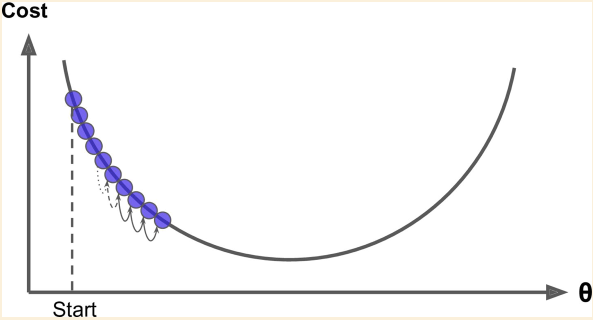
\includegraphics[width=6cm]{A2022.IDSEPC.RegressioneLineare/gd-2.png}
\end{center}



\begin{center}
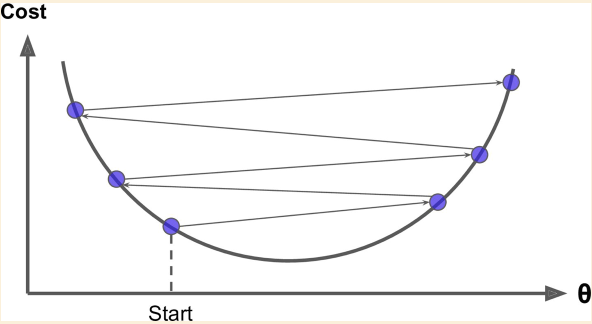
\includegraphics[width=6cm]{A2022.IDSEPC.RegressioneLineare/gd-3.png}
\end{center}



\end{frame}
%--------------%%--------------%%--------------%%--------------%%--------------%%--------------%
\begin{frame}
{\centerline{Pitfalls of Gradient Descent }}
\begin{center}
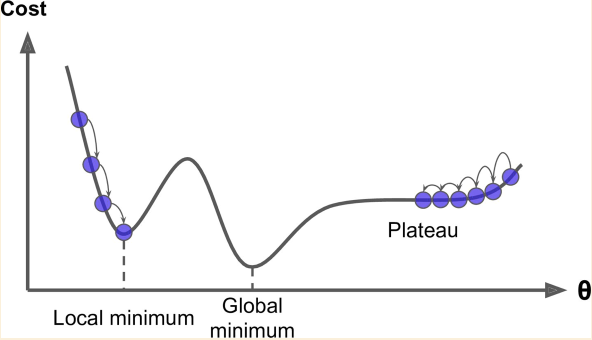
\includegraphics[width=8cm]{A2022.IDSEPC.RegressioneLineare/gd-4.png}
\end{center}
\end{frame}
% %--------------%%--------------%%--------------%%--------------%%--------------%%--------------%



% \begin{frame}
% {\centerline{}}

% \end{frame}

%--------------%%--------------%%--------------%%--------------%%--------------%%--------------%
\begin{frame}
{\centerline{Linear Regression and Machine Learning}}
Linear Regression is a statistical model developed in the field of Regression Analysis.

Later it was borrowed for the use of Machine Learning field.

\begin{table}[]
\centering
\caption{\textbf{Terminology difference}}
\begin{tabular}{|l|l|}
\hline
\textbf{Regression analysis} & \textbf{Machine Learning} \\ \hline
estimation, fitting          & training, learning         \\ \hline
regressors                   & features                   \\ \hline
response                     & target                    \\ \hline
\end{tabular}
\end{table}

\end{frame}


\begin{frame}
{ \centerline{References}}

1) \url{http://www.cs.umd.edu/~djacobs/CMSC426/Convolution.pdf}
\newline 

2) \url{https://www.researchgate.net/post/Difference\_between\_convolution\_and\_correlation}
\newline 

3) \url{https://www.tutorialspoint.com/signals\_and\_systems/convolution\_and\_correlation.htm}

\end{frame}


\begin{frame}
{\centerline{Domande?}}
\vspace{1cm}
\begin{center}
    \LARGE{Fine della lezione nove.}
\end{center}

\end{frame}


%----------------------------------------------------------------------------------------
\end{document}
